\documentclass[11pt, a4paper]{article}
\usepackage{graphicx}
\usepackage{amsmath}
\usepackage{listings}
\usepackage{placeins}
\usepackage{hyperref}
\usepackage[margin=1in]{geometry}
\usepackage[utf8]{inputenc}
\hypersetup{
  colorlinks   = true, %Colours links instead of ugly boxes
  urlcolor     = blue, %Colour for external hyperlinks
  linkcolor    = blue, %Colour of internal links
  citecolor   = red %Colour of citations
}

\title{\vspace{-2cm}%
  Kalman Filter Accelerator \\
  \vspace{0.5cm} \large EE2003 - Course Project}

\author{Arun D A (EE19B071), Sakthi Harish (EE19B054), Snehan (EE19B027)}
\date{December 2021}

\begin{document}

\maketitle

Git Repository: \url{https://git.ee2003.dev.iitm.ac.in/EE19B071/KalmanFilterAccelerator}
\section{Introduction}
Kalman filters are one of the most widely used algorithms. It produces estimates of hidden variables based on inaccurate and uncertain measurements. It also provides a prediction of the future system state based on past estimations. A common application is for guidance, navigation, and control of vehicles, particularly aircraft, spacecraft and ships positioned dynamically. Furthermore, Kalman filtering is a concept much applied in time series analysis used for topics such as signal processing and econometrics.
\newline
\newline In this project, we have implemented an Accelerator for a  Kalman Filter with 3 state variables. We have used a simulation of an Artix 7 FPGA board to analyse the hardware accelerator.  
\section{Project Description}
For this project, we have used Vitis HLS to generate the accelerator IP. The source code (in C) was generated using MATLAB coder. Using Vitis HLS, the design with floating point operations was produced with an AXI interface to integrate with Microblaze. The loop UNROLL directives were used to compute all iterations of the loops in parallel. Further, the floating point operations were converted to fixed point operations for a more optimized design. The exported IP was then integrated with Microblaze. 
\vspace{0.5cm}

\begin{figure}[!tbh]
\centering
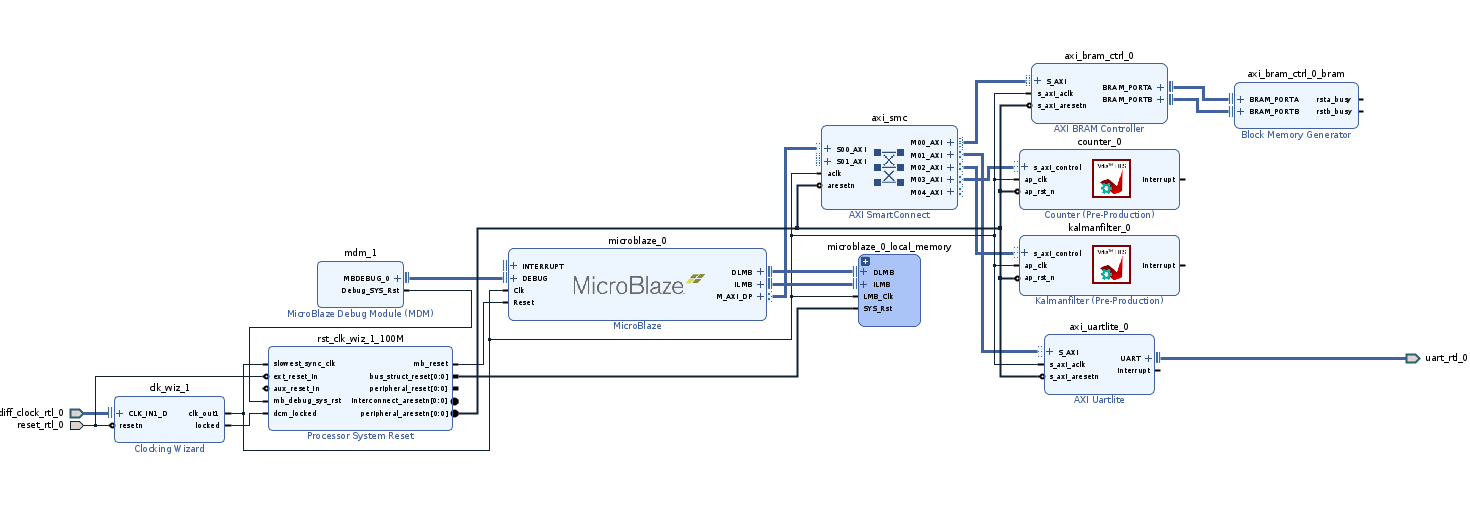
\includegraphics[scale=0.56]{bloc_design.png} 
\caption{Block design of Kalman Filter accelerator integrated with MicroBlaze}
\label{fig:fig_1}
\end{figure}
\vspace{0.5cm}
 For analysis, a performance counter IP was added to Microblaze. The performance of the hardware accelerator is then analyzed by comparing it to the software implementation in Microblaze(with and without FPU) and Intel i5 processor.
\newpage
\section{Results}

\subsection{Software Implementation}
{
\renewcommand{\arraystretch}{1.2}
\begin{table}[htbp]
    \centering
    \begin{tabular}{|c|c|c|c|}
    \hline
        Processsor & No. of cycles & Clock Speed & Total Time \\ \hline
        Microblaze without FPU & 415750 & 100MHz & 4157500 ns \\ \hline
        Microblaze with FPU & 187581 & 100MHz & 1875810 ns \\ \hline
        Intel i5 9300H & 4226 & 2.4GHz & 1761 ns \\
    \hline
    \end{tabular}
    \caption{Software Performance}
    \label{tab:my_label}
\end{table}
}
It can be seen that Microblaze (with FPU) takes nearly 44 times more cycles than Intel i5 to execute the same code. This can attributed to the lack of efficient methods for floating point multiplication and division in Microblaze and the poor memory access times due to the presence of a large number of arrays.
{
\renewcommand{\arraystretch}{1.2}
\FloatBarrier
\subsection{Hardware Implementation}
\begin{table}[htbp]
    \centering
    \makebox[\textwidth]{\begin{tabular}{|c|c|c|c|c|c|c|c|}
    \hline
         & Write & Read & Computation & Latency (Reported by HLS) & DSP & FF & LUT \\ \hline
        Floating Point & 120 & 108 & 365 & 215 & 70 & 10834 & 9078 \\ \hline
        \vtop{\hbox{\strut Floating Point}\hbox{\strut (Optimized)}} & 120 & 108 & 307 & 126 & 114 & 9597 & 9251 \\ \hline
        Fixed Point & 120 & 108 & 249 & 56 & 36 & 4767 & 5237 \\
    \hline
    \end{tabular}}
    \caption{Hardware Performance(@100MHz)}
    \label{tab:my_label}
\end{table}
}
\FloatBarrier
Upon converting floating points to fixed points, it can be seen that there is a large decrease in the resource usage and a significant increase in the performance. This is due to large no of resources required to perform floating point operation. For the fixed point implementation, it is also observed that only 373 clock cycles are taken in total when the counter is not called in between the write, compute and read operations. This means that (120+108+249)-373 = 104 cycles is used by two calls to the counter. Considering that we are calling the counter 4 times and assuming this delay is split evenly among the three parts, this would lead to an average delay of 70 cycles caused by the performance counter for each part, so (249-70)=179 cycles is used for computation. Taking into account HLS reports a latency of 56 cycles, (179-70)=123 cycles are used for setting the start bit and checking for completion of the computation. This delay can be reduced by using a faster AXI arbiter. The conversion of the u32 bits into a float data type and vice versa is responsible for the delay caused by the read and write operations.

\subsection{Conclusion}
As is evident from the results, the bottleneck in the hardware implementation is caused by the read and write operations and other delays caused by the AXI SmartConnect. The delays caused by the read and write operations can be reduced by using a processor that support more efficient floating point operations. The hardware implementation is around 1000x times faster than sofware run on Microblaze. Though the latency reported by HLS would mean that it is nearly 3x faster than software run on the Intel i5 processor, other delays result in the accelerator running at nearly the same speed as the software on the Intel processor. Though a speedup isn't achieved when compared to software run on modern processors, this is still useful as it consumes just 0.441W of power which makes it helpful for applications where low power usage is a requirement.


\section{Division of Work}

\begin{itemize}
    \item Executing test C code in Microblaze - Arun
    \item Generate C code for Kalman filter using MATLAB - Snehan
    \item Execute Kalman Filter code in Microblaze with and without FPU - Arun
    \item Design test ip with AXI in Vitis HLS and interface with Microblaze - Sakthi
    \item Adding and using a performance counter IP with MicroBlaze - Arun
    \item Mesaure performance of C code in Intel i5 processor - Snehan
    \item Design ip for kalman filter using floating point - Sakthi
    \item Add optimization directives - Arun
    \item Write C code in microblaze for using the kalman filter ip generated by HLS - Arun
    \item Change from floating point to fixed point - Arun
    \item Report - Sakthi, Arun, Snehan
    \item Video - Sakthi, Arun, Snehan
\end{itemize}


\section{References}

\begin{enumerate}
    \item \url{https://gitlab.com/chandrachoodan/teach-fpga/-/tree/master/01-fft/vivado/fft-sdk}
    \item \url{https://ieeexplore.ieee.org/document/7979508} 
    \item \url{https://digitalcommons.usu.edu/cgi/viewcontent.cgi?article=1784&context=etd}
    \item \url{https://en.wikipedia.org/wiki/Kalman_filter}
    \item \url{https://github.com/Neelam96/MicroBlaze-RTL-Simulation} (testbench.vhd)
\end{enumerate}

\end{document}
